% !TeX program = xelatex
% !TeX encoding = utf8
% !TeX root = RegT1E_HS22.tex

%% TODO: publish to CTAN
\documentclass[margin=normal]{tex/hsrzf}

%%%%%%%%%%%%%%%%%%%%%%%%%%%%%%%%%%%%%%%%%%%%%%%%%%%
% Packages
\usepackage{multicol}
\usepackage[export]{adjustbox}
\usepackage{bm}
\usepackage{color, colortbl}
\usepackage{trfsigns}
\usepackage{graphicx}
\usepackage{tabularx}
\usepackage{mathrsfs}
\usepackage{tikz}
\usetikzlibrary{plotmarks}

\usepackage{pgfplots}
\usepackage{lscape}


\usetikzlibrary{plotmarks}

\definecolor{TabularBackgroundColor}{rgb}{0.83,0.96,0.96}

%% TODO: publish to CTAN
\usepackage{tex/hsrstud}

%% Language configuration
\usepackage{polyglossia}

\setdefaultlanguage[variant=swiss]{german}

%% License configuration
\usepackage[
    type={CC},
    modifier={by-nc-sa},
    version={4.0},
    lang={german},
]{doclicense}


%%%%%%%%%%%%%%%%%%%%%%%%%%%%%%%%%%%%%%%%%%%%%%%%%%%
% Metadata

\course{Elektrotechnik}
\module{RegT1E}
\semester{Herbstsemester 2022}

\authoremail{joel.leirer@ost.ch}
\author{\textsl{Joël Leirer} -- \texttt{\theauthoremail}}

% did someone help you with this work?
\contributors{
  % do not forget to add yourself!
}

\title{\texttt{\themodule} Zusammenfassung}
\date{\thesemester}

%%%%%%%%%%%%%%%%%%%%%%%%%%%%%%%%%%%%%%%%%%%%%%%%%%%
% Document

\begin{document}

% use roman numberals for introductiory pages
\pagenumbering{roman}

\maketitle


% show the names of the people who contributed to this document.
% \section*{Contributors}
% \thecontributors

\section*{Lizenz}
\doclicenseThis

\clearpage
\tableofcontents

% actual content
\clearpage
\setcounter{page}{1}
\pagenumbering{arabic}

\section{Begriffe}
\begin{itemize}
      \item Prozess
            \begin{itemize}
                  \item Die Gesamtheit zusammenwirkender Vorgänge, welche durch
                        die Materie, Energie und Information
                        umgefort, transportiert und gespeichert wird.
            \end{itemize}

      \item System
            \begin{itemize}
                  \item Ist gegenüber der Umwelt abgegrenzt, hat Eingänge,
                        Ausgänge (und Zustand).
                  \item (LTI-/)LZI-Systeme: Lineare-ZeitInvariante Systeme
                        (Linearität gilt, System ist unabhängig von zeitlicher Verschiebung
                        --> DGL mit Konst. Koeff.)
            \end{itemize}

      \item Modell
            \begin{itemize}
                  \item Beschreibung von Systemen, wird genutzt für
                        Erklärung, Prognose, Gestaltung und Optimierung.
                  \item Es gibt kein "richtiges Modell",
                        ein Modell beschreibt ein System nur so genau wie nötig.
            \end{itemize}
      \item Modellieren
            \begin{itemize}
                  \item Teilsysteme erstellen und diese
                        in weitere Teilsysteme aufzutrennen.
                        So erhält man einfache Grundsysteme (Grundglieder),
                        welche sich einfach Mathematisch beschreiben lassen.
                        Zusätzlich kehern einige Teilsysteme in ihrer
                        Struktur oft wieder und können wiederverwendet werden.

                  \item Top-Down: System in Teilsysteme teilen
                  \item Bottom-Up: System aus Grundglieder aufbauen
            \end{itemize}
      \item Grundglieder
            \begin{itemize}
                  \item Kleinste Teilsysteme. Sie können weiter augeteilt werden in, siehe Abschnitt Grundglieder
            \end{itemize}
      \item Sprungantwort
            \begin{itemize}
                  \item Reaktion des Systems auf die Sprungfunktion. Siehe \refname{func}

            \end{itemize}
      \item Schrittantwort
      \item \begin{itemize}
                  \item Reaktion des Systems auf die Schrittfunktion. Siehe \refname{func}
            \end{itemize}
      \item Ausgleich
            \begin{itemize}
                  \item Prozesse ohne Ausgleich: Sprungantwort wächst Grenzenlos an
                  \item Prozess mit Ausgleich: Sprungantwort strebt endlichem Wert zu
            \end{itemize}

\end{itemize}




\begin{landscape}
      \subsection{Grundglieder}
      \begingroup
      \scriptsize
      \newcommand{\ImageWidth}{70pt}
      \begin{tabularx}{\linewidth}{|p{100pt}|p{160pt}|p{60pt}|p{80pt}|p{120pt}|p{80pt}|}
            \hline
            \textbf{Benennung}
             &
            \textbf{Funktion}
             &
            \textbf{UTF\textsuperscript{1}}
             &
            \textbf{Symbol}
             &
            \textbf{Sprungantwort}
             &
            \textbf{Plot}
            \\
            \hline
            \hline
            \textbf{P-Glied\textsuperscript{2}}
            \newline Proportionalglied
             &
            $y = K \cdot u$
             &
            $K$
             &
            \raisebox{-.5\height}{\includegraphics[width = \ImageWidth]{img/DIN-Symbole/Proportionalglied.png}}
             &
            Sprungantwort
             &
            \raisebox{-.5\height}{
                  \resizebox{\ImageWidth}{!}{%
                        \begin{tikzpicture}
                              % Grid
                              \draw[help lines,dashed] (0,0) grid (5,3);

                              % Axes
                              \draw[very thick,latex-latex] (0,3.25) node[left]{$y(t)$}
                              |- (5.25,0) node[below]{$t$};

                              % Plot function
                              \draw[ultra thick,teal] (-0.5,0) node[left,black](s0){$y(0)$}
                              -- ++(0.5,0)
                              plot[domain=0:5,
                                          samples = 50,
                                          smooth]({\x}, {2});
                        \end{tikzpicture}
                  }
            }
            \\
            \hline
            \rowcolor{TabularBackgroundColor}
            \textbf{I-Glied}
            \newline(Idealer Integrierer)
             &
            $y(t) = K \cdot \int \limits _{t=0} ^{t} u(\tau) d\tau + y(0)$
            \newline $\dot{y}(t) = K \cdot u(t)$
             &
            $K \frac{1}{s}$
             &
            \raisebox{-.5\height}{\includegraphics[width = \ImageWidth]{img/DIN-Symbole/Integrator.png}}

             &
            Sprungantwort
             &
            \raisebox{-.5\height}{
                  \resizebox{\ImageWidth}{!}{%
                        \begin{tikzpicture}
                              % Grid
                              \draw[help lines,dashed] (0,0) grid (5,3);

                              % Axes
                              \draw[very thick,latex-latex] (0,3.25) node[left]{$y(t)$}
                              |- (5.25,0) node[below]{$t$};

                              % Plot function
                              \draw[ultra thick,teal] (-0.5,0) node[left,black](s0){$y(0)$}
                              -- ++(0.5,0)
                              plot[domain=0:5,
                                          samples = 50,
                                          smooth]({\x},);
                        \end{tikzpicture}
                  }
            }
            \\
            \hline
            \textbf{Totzeit-Glied}
             &
            $y(t) = u(t-T_t)$
             &
            $e^{-s T_t}$
             &
            \raisebox{-.5\height}{\includegraphics[width = \ImageWidth]{img/DIN-Symbole/Totzeitglied.png}}
             &
            Sprungantwort
             &
            \raisebox{-.5\height}{
                  \resizebox{\ImageWidth}{!}{%
                        \begin{tikzpicture}
                              % Grid
                              \draw[help lines,dashed] (0,0) grid (5,3);

                              % Axes
                              \draw[very thick,latex-latex] (0,3.25) node[left]{$y(t)$}
                              |- (5.25,0) node[below]{$t$};

                              % Plot function
                              \draw[ultra thick,teal] (-0.5,0) node[left,black](s0){$y(0)$}
                              -- ++(0.5,0)
                              plot[domain=0:5,
                                          samples = 100,
                                    ]({\x},{ (\x<=2) * 0  + (\x>2) * 2});
                        \end{tikzpicture}
                  }
            }
            \\
            \hline
            \rowcolor{TabularBackgroundColor}
            \textbf{PT\textsubscript{1}-Glied}
            {
                  \tiny \newline K: Verstärkung
                  \newline T: Zeitkonstante
            }
             &
            $ T\dot{y} + y = K u(t)$
            \newline $T= \frac{1}{K_I \cdot K_P} $
            \newline $K = \frac{1}{K_P}$
             &
            $\frac{K}{1+T_s}$
             &
            \raisebox{-.5\height}{\includegraphics[width = \ImageWidth]{img/DIN-Symbole/PT1-Glied.png}}
             &
            Sprungantwort
             &
            \raisebox{-.5\height}{
                  \resizebox{\ImageWidth}{!}{%
                  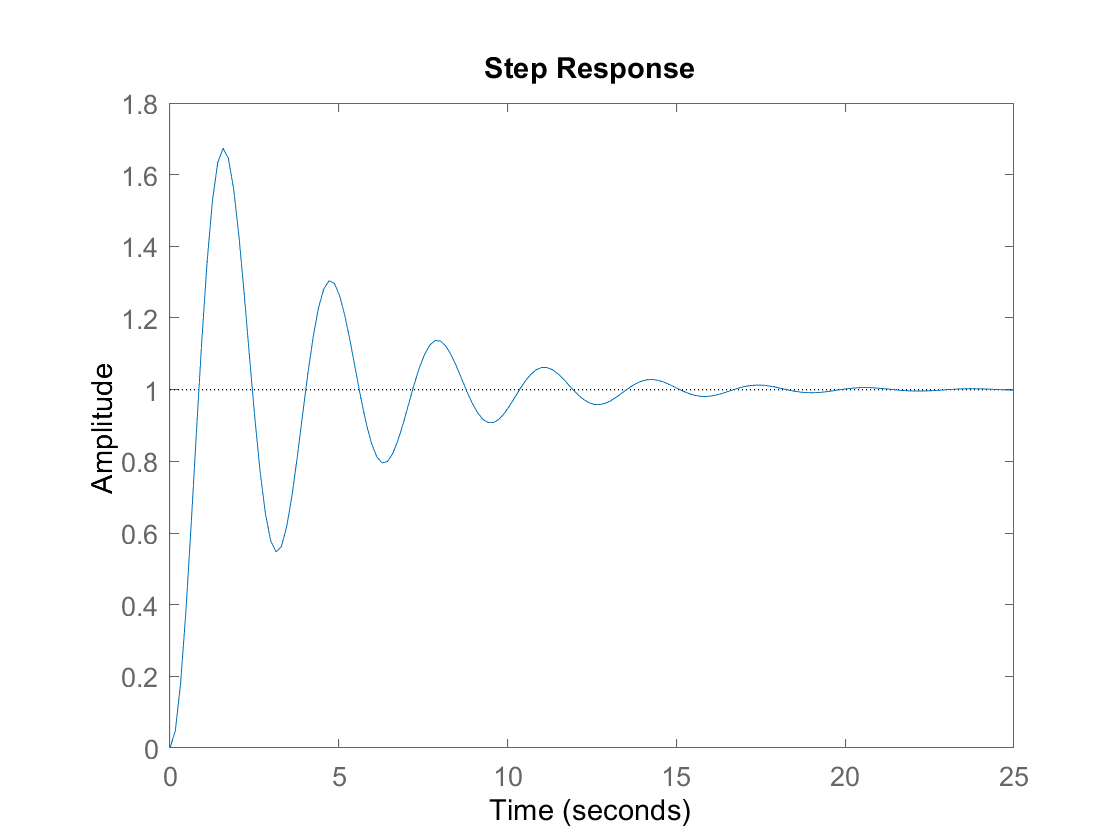
\includegraphics{matlab/PT2.png}


                        \begin{tikzpicture}
                              % Grid
                              \draw[help lines,dashed] (0,0) grid (5,3);

                              % Axes
                              \draw[very thick,latex-latex] (0,3.25) node[left]{$y(t)$}
                              |- (5.25,0) node[below]{$t$};

                              % Plot function
                              \draw[ultra thick,teal] (-0.5,0) node[left,black](s0){$y(0)$}
                              -- ++(0.5,0)
                              plot[domain=0:5,
                                          samples = 50,
                                          smooth]({\x},{2.5*(1- exp(-(\x)))});
                        \end{tikzpicture}
                  }
            }
            \\
            \hline
            \textbf{PT\textsubscript{2}-Glied}
            {\tiny
                  \newline K: Verstärkung
                  \newline T: Zeitkonstante
                  \newline $\zeta$: Dämpfungskonstante
            }
             &
            $T^2 \cdot \ddot{y}(t) + 2 \zeta T \cdot \dot{y}(t) + y(t) = K \cdot u(t)$
            \newline $y(t) = K \cdot x(t) + T^2 \cdot (-\ddot{y}(t)) - 2 \zeta T \cdot \dot{y}(t)$
            {\tiny
                        \newline $\zeta = \frac{h}{\sqrt{h^2 + \pi^2}}$
                        \newline $h = \log(\frac{y_m}{y_{\infty}})$
                  }
             &
            $\frac{K}{T^2 + s^2 + 2 \zeta T s + 1}$
             &
            \raisebox{-.5\height}{\includegraphics[width = \ImageWidth]{img/DIN-Symbole/PT2-Glied.png}}
             &
            $KA(1+e^{\sigma t}(-cos(\omega t) + \frac{\sigma}{\omega}sin(\omega t)))$
            {\tiny
                        \newline $\omega = \frac{2\pi}{T_m}$
                        \newline $K = \frac{y_{\infty}}{A} $
                        \newline $\sigma = \frac{h\omega}{\pi}$
                  }
             &
            \raisebox{-.5\height}{
                  \resizebox{\ImageWidth}{!}{%
                        \begin{tikzpicture}
                              % Grid
                              \draw[help lines,dashed] (0,0) grid (5,3);

                              % Axes
                              \draw[very thick,latex-latex] (0,3.25) node[left]{$y(t)$}
                              |- (5.25,0) node[below]{$t$};

                              % Plot function
                              \draw[ultra thick,teal] (-0.5,0) node[left,black](s0){$y(0)$}
                              -- ++(0.5,0)
                              plot[domain=0:5,
                                          samples = 50,
                                          smooth]({\x},{2.5  *   (1- exp(-3*(\x))  *  (- cos(deg(1.9848*\x)) + (-3/1.9848)*sin(deg(1.9848*\x)))  });
                                          %KA = 2.5, Sigma = -3, Omega = 1.9848
                        \end{tikzpicture}
                  }
            }
      \end{tabularx}
      \tiny{
            \\
            1. UTF = Übertragungsfunktion (Laplace)\\
            2. Proportionalglied ist einziges Statisches glied.\\
      }
      \endgroup
      \normalsize
\end{landscape}

\section{Klassen von Systemen}


\newpage
\input{include/Integraltransformationen/Integraltransformationen.tex}
%needs Packages:
% - \usepackage[export]{adjustbox} for  "valign=t"

\section{Wichtige Funktionen}
\begin{tabular}{p{5cm} p{12.5cm}}
  \includegraphics[width = 5cm, valign=t]{include/Wichtige Funktionen/img/Sprungfunktion.png} &
  \textbf{Sprungfunktion (Heaviside)}
  \footnotesize
  Normierter Einschaltvorgang
  $$H(t) = \begin{cases}
               0 \textrm{ für }  t<0,                                                                      \\
               [\frac{1}{2} \textrm{ für }  t = 0,] \textrm{ \tiny(nicht immer vorhanden; dann 1 für t=0)} \\
               1 \textrm{ für }  t >0.
             \end{cases}   $$
  \\
  \includegraphics[width = 5cm, valign=t]{include/Wichtige Funktionen/img/Impulsfunktion.png} &
  \textbf{Diracimpuls} \tiny (auch Impuls-/Deltafunktion, Delta-Distribution)
  \footnotesize \newline
  Unendlicher kurzer normierter Impuls mit unendlicher Amplitude
  $$\int\limits _{-\infty} ^{+\infty} f(t) \cdot \delta (t-t_0) dt = f(t_0) \;
    \int\limits _{-\infty} ^{+\infty} f(t) \cdot \delta (t) dt = f(0) \;
    \int\limits _{-\infty} ^{+\infty} \delta (t) dt = 1$$
  TODO: \includegraphics[width=5cm]{include/Wichtige Funktionen/img/Eigenschaften _delta.png}   \\
  \includegraphics[width = 5cm, valign=t]{include/Wichtige Funktionen/img/Signumfunktion.png} &
  \textbf{Signumfunktion} (Vorzeichenfunktion)
  \footnotesize
  $$sgn(t) = \begin{cases}
                 -1 \textrm{ für }  t<0,  \\
                 0 \textrm{ für }  t = 0, \\
                 1 \textrm{ für }  t >0.
               \end{cases}   $$                                                           \\
  \includegraphics[width=5cm, valign=t]{include/Wichtige Funktionen/img/Rampenfunktion.png}   &
  \textbf{Rampenfunktion}
  \footnotesize
  $$r(t) = \begin{cases}
               0 \textrm{ für } t \leq 0, \\
               t \textrm{ für } t > 0.
             \end{cases}$$                                                           \\
  \includegraphics[width=5cm, valign=t]{include/Wichtige Funktionen/img/Rechteckimpuls.png}   &
  \textbf{Rechteckimpuls}
  \footnotesize
  $$p_a(t) = u(t+a)-u(t-a)= \begin{cases}
                                1 \textrm{ für } |t| < a,           \\
                                \frac{1}{2} \textrm{ für } |t| = a, \\
                                0 \textrm{ für } |t| > a.
                              \end{cases} $$                                 \\
  \includegraphics[width=5cm, valign=t]{include/Wichtige Funktionen/img/Dreieckimpuls.png}    &
  \textbf{Dreieckimpuls}
  \footnotesize
  $$\Lambda(t) = \begin{cases}
                     1 - \frac{|t|}{a} \textrm{ für } |t| < a \\
                     0 \textrm{ für } |t| \geq a
                   \end{cases}$$                                       \\
  \includegraphics[width=5cm, valign=t]{include/Wichtige Funktionen/img/SincFunktion.png}     &
  \textbf{Sinc-Funktion}
  \footnotesize
  $$sinc(t) = \frac{sin(t)}{t} \forall t$$                                                                                     \\
\end{tabular}

\input{include/LTI-Systeme/LTI-Systeme.tex}

\section{Tabellen}

\subsection*{Blockschaltbilder MatLab}
\begin{tabular}{|c|c|c|c|c|}
      \hline
      \textbf{Summierer}                                            &
      \textbf{Differenzbilder}                                      &
      \textbf{Konstante}                                            &
      \textbf{Proportionalglied}                                    &
      \textbf{Integrierer}                                            \\
      \includegraphics[]{img/matlab/sum_block_icon.png}             &
      \includegraphics[]{img/matlab/difference_block_icon.png}      &
      \includegraphics[]{img/matlab/constant_block_icon.png}        &
      \includegraphics[]{img/matlab/gain_block_icon.png}            &
      \includegraphics[]{img/matlab/integrator_block_icon.png}        \\
      \hline
      \textbf{Totzeitglied}                                         &
      \textbf{Differenzierer}                                       &
      \textbf{}                                                     &
      \textbf{}                                                     &
      \textbf{}                                                       \\
      \includegraphics[]{img/matlab/transport_delay_block_icon.png} &
      \includegraphics[]{img/matlab/derivative_block_icon.png}      &
      \\
      \hline
\end{tabular}
\end{document}
